\section{SMURF Pipeline}

The proposed pipeline for composing music with SMURF is demonstrated in Figure~\ref{fig:pipeline}. 
The composer creates serial music by first writing a SMURF program, which will be 
compiled by our SMURF compiler to generate a C program with OpenGL. Then the gcc compiler 
and assembler are used to generate a music score with which musicians can play. 


\begin{figure}
	\centering
	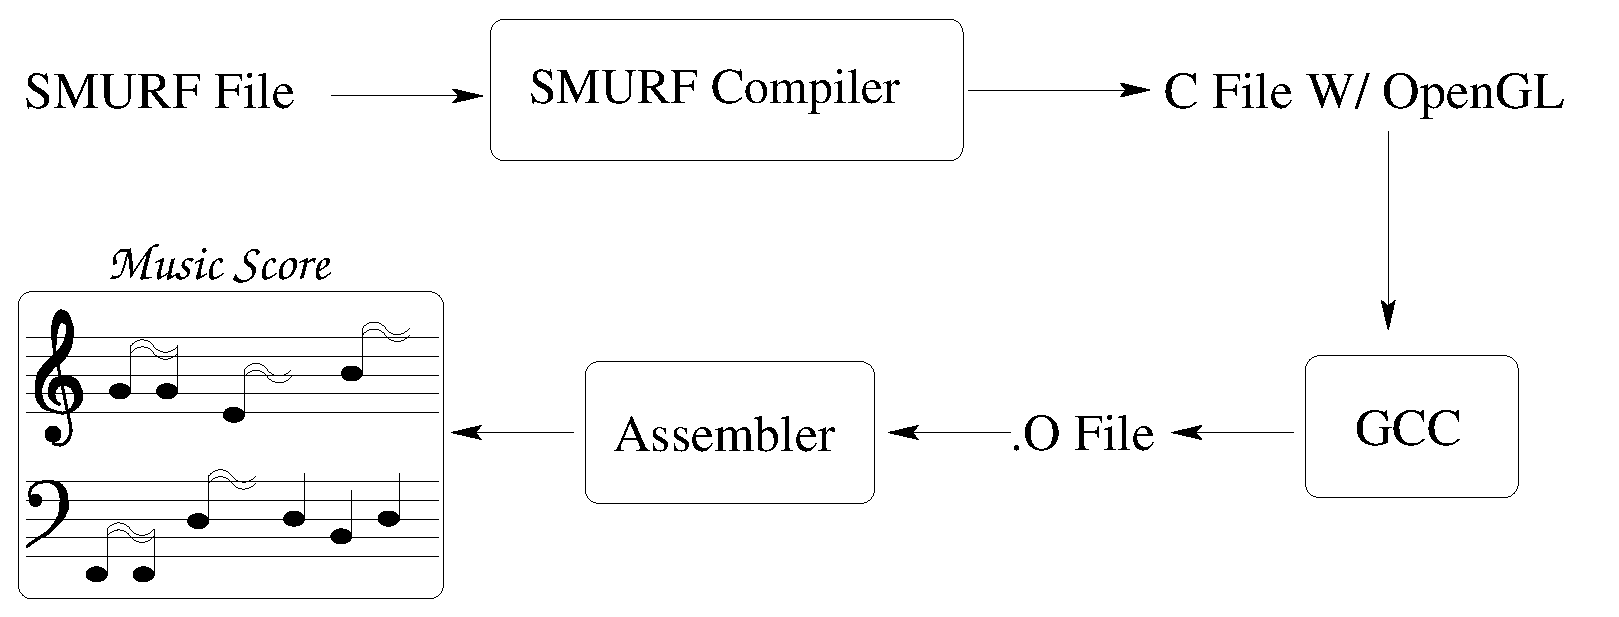
\includegraphics[width=0.75\textwidth]{figures/pipeline}
	\caption{SMURF pipeline for composing serialist music}
	\label{fig:pipeline}
\end{figure}
